\documentclass[11pt, twoside]{report}
\usepackage[margin=.5in]{geometry}
\usepackage{indentfirst}
\usepackage{hyphenat}
\usepackage{hyperref}
\usepackage{graphicx}
\usepackage{tabto}


\makeatletter
\renewcommand{\thesection}{%
  \ifnum\c@chapter<1 \@arabic\c@section
  \else \thechapter.\@arabic\c@section
  \fi
}
\makeatother

\newcommand{\refapp}[1]{\textsuperscript{[\ref{#1}]}}

\title{An Overview of the ROBERT Platform for the Purpose of Autonomous Agricultural Data Acquisition and Actuation
\author{Hunter Halloran, William Snapp, Kevin Koffroth, Michael Starks, \\Caroline Lassiter, Cole Sterck, John Bare, Tommy Anton, Jake Alford\thanks {Mentored by Changying "Charlie" Li, Ph.D., Fred Beyette, Ph.D, and Jawad Iqbal}\textsuperscript{,}\thanks{Sponsored by the University of Georgia College of Engineering, the Bio-Sensing and Instrumentation Lab, AGCO, and IGUS}} } 
\date{5 July, 2020}



\begin{document}
\begin{titlepage}
\maketitle
\end{titlepage}

\newpage
\setcounter{tocdepth}{3}
\raggedbottom
\tableofcontents
\newpage

\section{Introduction}
\subsection{Need In Agriculture and Approach}
While last year this team faced the issue of designing the robot only to meet the task of the competition and failing to consider a net benefit to agricultural robotics, this robot was designed targeting real world surrogates to represent real needs in autonomous field robotics. This system was designed as a modified shadow of the Bio-Sensing and Research Lab’s MARS robot, a system designed to drive over crop rows to image on all sides with a 4-wheel steering mechanism for absolute positioning control. In the shrunken scale, the competition robot was able to benefit from design considerations already realized physically from the MARS platform while being able to more rapidly consider other methods in the miniature construction, allowing for the possibility of multi-row processing in parallel without needing to build a full robot in full crop-field size. 

This platform demonstrates a positive impact for autonomous field platforms due to the aforementioned considerations. By using a large form factor capable of driving over crop rows, the system can have more opportunities for data acquisition in various positions, by either taking multiple images and other data readings simultaneously or being able to readjust a single camera until a suitable position for data accumulation has been found. Further, by having an extensible platform created with the intention of possible modification due to modularity as an internal design requirement, other systems can also be added, such as actuation platforms demonstrated in this robot as the seed dispensers. In this case, the modular nature comes from replaceable acrylic panels capable of being removed and replaced with a new panel with required mount points, but as this system exists as a concept to be scaled as the MARS system, aluminum extrusion is the conceptual equivalent for new mount points.

\subsection{Definition of Design Objectives}
The overall robotics system implemented multiple internal requirements beyond the necessary scope of the competition for the purposes of creating a generalized system to demonstrate the abilities of a platform rather than designing only for the 2020 ASABE Student Robotics Challenge. For this reason, molecularity and efficiency were large goals for the design. It was chosen to create an expanding assembly to be able to compromise between a desire to accumulate data for the play-field in a parallelized manner while meeting the competition requirements of beginning within a one square cubic foot volume. Due to a desire to mirror other agricultural robotics systems from the University of Georgia as a miniaturized testbed, the design needed to include a 4-wheel steering design with four individually steerable wheels to mimic the MARS platform and Mini-Flowerbot designs from B-SAIL\footnote{The Bio-Sensing and Instrumentation Lab}, as well as being able to demonstrate a more realistic means of navigation over a crop field rather than omnidirectional wheels which would not be able to function in a soil environment. 

The design of the overall system also needed to be extensible to be able to include a suite of sensors and actuators to achieve the required task for the challenge. In this case, the requirement is the mounting of cameras for both plant health detection and line following, as well as actuators for the dispensing of seeds for missing crops. An internal requirement was created of designing using primarily acrylic sheets to allow for rapid prototyping with locked 2D pieces rather than a slower process of 3D printing each necessary component. For the purposes of distinguishing between stressed and unstressed plants a visual identification system is required using cameras and image processing. It was pushed to make use of a deep learning application to complete this to align more closely with actual field robotics.

\section{Hardware Description\refapp{app:mech}}
\subsection{Overview}
For the mechanical design for the robot, the team wanted to optimize for speed, accuracy, and weight of the robot.  The design process began prior to the release of the rules with the design of a simple testbed for line following and navigation prototyping.  The testbed design used a square of aluminum extrusion with stepper motors for actuation and Mecanum wheels to move forwards and backwards as well as strafe sideways.  This design had to be abandoned as soon as rules were released due to the heaviness of the motors as well as the aluminum extrusion.  After this model was made, the team decided to use a body made of laser-cut acrylic moving forward, due to the customizability, the ease of use, and the weight reduction provided by a lighter and thinner material.

The first competition-specific design built was a panel-based design, with cameras and droppers mounted on each side.  The cameras were mounted on panels that deployed out sideways, blocking out ambient light and shining LED lights to provide optimal lighting for analysis. This design was decided on due to its ability to scan 2 rows at once, allowing the system to only make 2 passes through the course, instead of 4.  

The design process for this was set in 2 phases, with a phase 1 that was mainly for gauging the capabilities of both our hardware and software, and phase 2 based around building an expanding design that pushed our capabilities and maximized our points and efficiency.  Separate chassis designs were essential to developing different mechanical subsystems.

\subsection{Dropper Progression}
The first dropper iteration was far too heavy, and used springs to actuate the dropping mechanism.  This system was far too heavy to prevent strain on the chassis of the robot, so we redesigned the dropper.  We narrowed the column that holds the seeds and reduced the body significantly, while lowering the infill in the 3D print in order to lighten it further.  The bottom portion was narrowed considerably and thinned out, and the pivot between the upper and lower was redesigned to use a smaller bolt, reducing the weight by narrowing the bolt from a ¼ inch bolt to an M2 bolt.  The spring was also changed to a rubber band, increasing consistency and further reducing weight.  The distance required to actuate the mechanism was also reduced.

Mechanical design went through many iterations before settling on a dropper design.  We wanted to be able to fill every seed deposit, and we wanted a design that could differentiate between an empty space and a plant without the need for any computation, in order to save computational power and cut overall time.  We accomplished this with a dropper assembly with an upper and lower portion.  The upper portion holds the “seeds” and connects the dropper assembly to the robot.  The lower assembly is spring-loaded at the joint with the robot and the joint with the lower assembly, and is engaged when it collides with the cups where the seeds belong.  It pulls the lowest seed from the column through an opening in the holder and drops it into the seed cup, before being stopped by the mechanism’s end piece and engaging the stronger inner spring that pushes the dropper past the cup.  Should it collide with an already grown corn stalk, the upper portion will make contact first, and the dropper will simply slide off without engaging the lower portion.

The droppers had to be fixed to make them slightly longer and attached to a Dynamixel motor.  The motors are used to measure resistance, and contact with a plant will cause the cameras to take a picture to determine the state of the plant.  
The last major change made to the chassis was the replacement of the drawer slides.  The first drawer slides we chose didn’t extend smoothly or fully extend without extra force.  We changed them to a different drawer slide.  The sides also had a tendency to recompress during the course of each run, so some 3D printed locks were made to lock open the side sections once they expanded.

The dropper length had to be further adjusted after this due to the minor extension difference in the drawer slides.  This was to enable them to more accurately hit each empty spot. To further increase the effectiveness of each dropper, the bottom portion was changed from a straight piece pressing against each cup to a cupped section that wraps around each seed-holding cup.  This would allow the position of each seed to accurately drop directly into the center of each cup, preventing them from falling out or getting jammed.  We also adjusted the inside dropper connecting section to curve away from the body sooner, allowing them to avoid the camera mount on the bottom of the robot.

\subsection{Drive System Progression}
The drive system we used was based around mecanum wheels at first(wheels made up of slanted rollers placed along the edge of the wheel, allowing for forward and backward movement, as well as sideways movement by engaging the motors in opposite directions).  These wheels were satisfactory for making a test platform, but after some testing we realized that they introduced too much slip, and changed to a 360 degree steering system, where there are two motors attached to each wheel, one to control wheel rotation and one to control direction.  The motor that controls wheel rotation is mounted such that the axis of rotation passes through the center of the point of contact for the wheel, meaning that they rotate exactly on axis, preventing slip while allowing the wheels to rotate the body or strafe in any direction at any time.  This system makes navigating the course much easier and provides more options for movement.

The first iteration of the 360 degree steering had bulkier motor mounts than necessary and used wheels that didn't have enough grip to accurately navigate the course.  To fix this, we slimmed down the motor mounts and thinned the walls, and purchased new wheels with smooth rubber designed to eliminate slip.  

\subsection{Chassis Progression}
After the design of the first phase of our chassis, we decided that in order to increase the speed of each run, we should move to an expanding design that could scan all four rows at once.  To accomplish this, our chassis is constructed of three main portions.  An inner portion houses the main electronic components, holds the droppers and cameras for the two inside rows.  This section is held up by two outer sections that hold the driving mechanism and the outside droppers and cameras.  The driving mechanism is used to expand the robot without the need for extra actuation.  The robot begins in the corner, and the two outer sections drive to their expanded location, while holding up the central section with drawer slides.  The closest outer section navigates to between the first and second row, and the other outer section navigates to between the third and fourth wall, while suspending the center section over the area between the second and third rows.  The cameras are not able to be rigidly mounted in place due to the size constraints of the robot.  Instead of using panels, we decided to have the cameras mounted on mounts that deploy via smaller servos at a 45 degree angle to the angle of the ground.  

\section{Software Overview\refapp{app:nav}\refapp{app:vision}\refapp{app:system}}
\subsection{Navigation and Drive System}
Using OpenCV, a common image-processing suite, the camera identifies contours, a summation of points with similar shade/intensity. This process entails converting the frame to grayscale so that different shades detected within the frame, and whose colors fit within the chosen shade range (black/dark grey), can be identified. This range is determined by passing in a range of RGB values. Based on the list of contours found in the frame, the robot finds the largest of these contours and uses them to identify the black tape. To account for any light reflecting off of the tape, the Robot considers a range of greys rather than solely black to detect the maximum number of points in the frame.

The angle is identified by determining the center x-coordinate of the frame making the center of the frame the robot’s focal point. The robot then determines the top middle coordinate, within the contour, by observing the x-values of coordinates with  lower y-values (Insert diagram of contour with origin labeled)in the contour closest to the front portion of the tape. Then, the difference between the robot’s focal point and the tape’s top-center coordinate is found, storing the distance as x and y values. Using trigonometry, the angle can be calculated with the gathered values, converted to degrees, and returned. 
The translation of the robot, off of the tape, is identified by finding a rectangle that approximates the shape of the tape. The contours of  the approximation are filtered to those concentric with the focal point of the camera, we compare it to the center point of the frame, calculating the horizontal distance between the robot’s focal point and the center of the tape, allowing us to determine the distance that the robot needs to travel, to realign its focal point with the center of the tape.

The Robot navigates the field guided by a path defined by Black electrical tape. The position of the Robot is a combination of its angular and linear positions. Using a polar coordinate system allows corrections to be completed in two distinct operations: angle corrections to fix heading and linear correction to fix drift laterally from the desired path. The Robot aims to maintain a heading +/- .3 degrees from zero and +/- .3 inches from the centerline To reduce the impact that path correction has on completing the task, angle correction is completed before lateral corrections.

Angular correction is done using center axis turning. Center axis turning has all of the Robot’s wheels turn normal to the radius of the Robot moving in the same direction. The current angle of the Robot is retrieved from the Line Tracking code and the Robot moves in the opposite direction of the current angular offset to correct the heading to be parallel to the Tape path. The Robot rotates in place, realigning with the crop rows before calculating the lateral correction path.

Correcting the heading of the Robot by turning on the center axis simplifies the lateral correction procedures. The lateral correction vector is calculated assuming the Robot’s heading is parallel to the taped path, the distance from the path is retrieved from the Line Tracking code, and a correction path is calculated using the error distance and a four-inch run to maintain forward motion while correcting the path. Lateral correction uses Crab Steering, moving the wheels to create a vector in the desired direction instead of moving the entire robot corrects faster and minimizes alignment error with crops. 

\subsection{Image Capture and Preprocessing}
Classifying each germination position on the competition board, was broken into two sub-tasks: capturing and preprocessing image data for each position, and constructing a reliable method of detecting the germination status with said image data. Image capture and processing, used OpenCV  allowing us to programmatically capture and edit images taken by the cameras on the robot. We crop the images to reduce misidentification and generally restrict the data our detection system process to only include the target germination position. For our capture system to work, we needed a method of reliably detecting when to take a picture, i.e. when our camera is lined up with the next germination position\refapp{app:uncrop}\refapp{app:crop}. We initially prototyped a system using simple limit switches and a coffee stir. This worked okay when testing off of the robot, but when the stalks came in rapid succession, the limit switch never had enough room to release, causing several missed triggers\refapp{app:ogtrig}. The next iteration of the trigger system utilized the existing mechanical dropper design\refapp{app:TODO}, along with a ROBOTIS Dynamixel\footnote{Dynamixel motors are a brand of particularly capable smart actuators. (\url{https://www.robotis.us/dynamixel/})} motor to create a spring-like trigger system that would capture an image after a set force is applied to the mechanical dropper. We did this by utilizing some of the smart actuator\footnote{A smart actuator is an actuator with a microcontroller(s), sensor(s), and communication unit(s). It typically communicates with a host device to deliver various data such as position, load, sensor data, etc.} capabilities of the Dynamixel motors, one of which is a readable ‘present load’ value which represents the electric current through the motor at that time. Since the current sensing works by measuring any current through the motor, back-driving them also changes the ‘present load’ value, making it useful as a torque sensor. Using this functionality, we were able to model the Dynamixel as a spring, letting the stalk back drive the motor and trigger the camera, then when force is no longer being applied, the motor moves back to its original position to sense the next stalk\refapp{app:dyntrig}.

\subsection{Image Classification}
The detection software uses the post processed images from the cameras to classify each image by germination status. Initial efforts to accomplish this used a simple OpenCV script which would count the number of Yellow, Green, and White pixels in an image, and output that as a percentage\refapp{app:ogimg}. This worked well enough in simple cases, but occlusion\footnote{Occlude: to shut in, out, or off. (\url{https://www.dictionary.com/browse/occlude?s=t})} of the target crop made detection inaccurate. While we could have developed more advanced computer vision techniques using OpenCV, we decided to use a machine learning approach as we had an interest in learning it. 

Explorations into neural network toolkits lead us to the TensorFlow\footnote{A free and open-source software library developed by Google and implemented frequently in machine learning applications. (\url{https://www.tensorflow.org/})} ecosystem, which is a free and open-source software library developed by Google and implemented frequently in machine learning applications. To assist us with the task of training our image classifier, we layered Keras\footnote{Keras is the high-level neural network API used in the TensorFlow ecosystem, it is included with TensorFlow when you install it on your system. (\url{https://www.infoworld.com/article/3336192/what-is-keras-the-deep-neural-network-api-explained.html})} and SciKit-learn\footnote{SciKit-learn is another high-level neural network API. While it can be used to create models, we are using it to manage the training of our neural network, collect and display metrics, and perform model selection. (\url{https://scikit-learn.org/stable/index.html})} on top of TensorFlow so that we could take advantage of their user-friendly APIs. Thanks to the open-source nature of these frameworks, it was easy for us to get started learning and experimenting using guides and tutorials as resources to achieve our goal of an accurate custom image classifier. Implementing our code using Anaconda\footnote{Anaconda is an easy to use Python workspace/environment manager. (\url{https://www.anaconda.com/})} and Jupyter Notebooks\footnote{Jupyter Notebooks is an open-source web application that allows you to create and share documents that contain live code, equations, visualizations and narrative text. This is especially useful for neural network training, as the code can be segmented and run arbitrarily, eliminating the need to rerun code that already executed without issue, and saving heaps of time in the process. (\url{https://jupyter.org/})} allowed for quick prototyping and development, as Anaconda made managing Python environments a breeze, and Jupyter Notebooks allowed us to break our modeling/training code into smaller segments, an essential for debugging machine learning applications. 

The training for our model began by first collecting and organizing our training data. We did this by generating a random competition board using the competition\_gui script, and taking 10 pictures of each position on the board, making sure to rotate the plants slightly between pictures. To more easily capture and organize the data, we developed a small OpenCV script which would capture, crop, and save images to predefined directories. This script was intentionally made to emulate how the photos would be captured and processed on the robot to eliminate variability in our model\refapp{app:util}. The images were sorted into yellow, green, and open directories to represent the three classes in our classification model. We used SK-learn’s LabelEncoder and One-Hot Encoding to organize the input and output variables into numeric form. Our data set was then split into a training set and validation set with a 1:4 ratio. As the names imply, the training set is used to train the neural net, while the validation set is used to test accuracy. A Keras Sequential model was then built out and image augmentation was implemented to prevent overfitting of the model. We then trained the model for 1500 epochs where we achieved a ~99\% validation accuracy\refapp{app:model}.

This gave us confidence in the ability of the model to correctly predict the plant status, but we were concerned with the speed of the neural net on the robot’s Single Board Computer. To run the classifier on the Google Coral Dev Board, we needed the model to be converted into a TensorFlow (TF) Lite model. Fortunately, the TF library includes a function to convert the Keras model to a TF Lite model. Running the neural net with TF Lite on the Coral Board resulted in classifications performed in half the time compared to the Raspberry Pi.

\subsection{Software System Integration}
For performance reasons, and to more easily integrate all of our software systems, the team decided to utilize the Python multiprocessing module\footnote{The multiprocessing module provided by Python is an easy to use API for creating and managing multiple Python Interpreters. (\url{https://docs.python.org/3/library/multiprocessing.html})} to easily leverage parallel programming. While doing initial testing of the navigation and vision systems, it became clear that having a true state machine would have significant performance impacts, because Python is an interpreted language\footnote{A summary of the advantages and disadvantages of Interpreted Languages can be found here. (\url{https://en.wikipedia.org/wiki/Interpreted\_language})}, making it significantly slower than something ‘native’ or compiled like C/C++, which runs almost directly on the hardware. The team initially tried using the Python threading module\footnote{The threading module provided by Python is an easy to use API for creating and managing separate threads within a process. (\url{https://docs.python.org/3/library/threading.html})}, which enables a developer to have separate ‘threads’ or pieces of code running concurrently on the same Python interpreter. After further testing, it became apparent that threading would still be a performance bottleneck, as Python has something called the Global Interpreter Lock\footnote{Description of the Global Interpreter Lock. (\url{https://en.wikipedia.org/wiki/Global\_interpreter\_lock})} which locks code execution to one thread at a time. It was at this point that the team turned to the Python multiprocessing module, which allows all of the subsystems to be executed in parallel, providing the modularity and performance the team was looking for. Some of the functionality of the robot requires the separate processes to communicate\refapp{app:sysdiag}. Fortunately, the multiprocessing module has solutions for this, implementing easy to use wrappers for the standard Pipe and Shared Memory APIs provided by the Operating System\footnote{A short summary of different interprocess communication methods in Linux (\url{https://opensource.com/article/19/4/interprocess-communication-linux-storage})}.

To effectively coordinate the various subsystems, the team organized them into a class structure, with each class having a constructor, any helper methods it may need, and a ‘Run’ method which would run code in a separate process, if need be. 

This class structure shines when the team started thoroughly testing the platform’s subsystems, as all they had to do was import a module’s respective code, set up any extra imports or code, set up the multiprocessing, and run the systems in question. This made independently validating all of the software a simple endeavour and ensured it would be executed in precisely the same way no matter if it was a test script, or the actual robot bringup script.


\section{Results}
Todo


\setcounter{secnumdepth}{3}
\section{Appendices}
\renewcommand{\thesubsection}{\Alph{subsection}}
\renewcommand{\thesubsubsection}{\Alph{subsection}.\arabic{subsubsection}}

\subsection{Mechanical} \label{app:mech}
\subsubsection{Parts List} \label{app:parts} 
\begin{center}
\nohyphens{
		\begin{tabular}{| p{3cm} | c | p{3cm} | p{5cm} |}
		\hline
			Part & Quantity & Material & Purpose \\ \hline 
			Dynamixel AX-12 & 12 & Servo Motors & Actuating motors used for drive system and sensing for droppers \\ \hline		
			Acrylic Sheets & 9 & Acrylic & Laser cut acrylic used for lightweight expanding chassis design \\ \hline 
			Andymark 2” Stealth Wheels & 4 & Rubber/Plastic & Provide necessary traction while navigating the course \\ \hline 
			Motor Mounts & 4 & 3D Printed PLA & Allow necessary mount points for 360 degree steering \\ \hline 
			Drawer Slides & 4 & Aluminum & Enable the expanding mechanism to expand linearly without sacrificing structural integrity or introducing excessive bend \\ \hline 
			Logitech Webcam Assembly & 1 & Electronic Component & Downward facing camera used for line following and course navigation \\ \hline 
			Arducam & 4 & Electronic Component & Used to scan rows of corn and record data \\ \hline 
			IGUS Cable Organizers  & 2 & Plastic & Used to secure and hold wires while expanding and navigating the course \\ \hline 
			Camera Mounts  & 5 & 3D Printed PLA & Used to secure cameras in place \\ \hline 
			Smrza Micro Servo Motors & 4 & Servo Motors & Used in expanding process to position cameras correctly \\ \hline 
			Google Coral Dev Board & 1 & Electronic Component & Acts similarly to an Raspberry Pi but with tensor processing units to accelerate machine learning applications \\
		\hline	
		\end{tabular}
}
\end{center}
	

\subsection{Navigation and Drive System} \label{app:nav}
\subsubsection{TODO}


\subsection{Vision System} \label{app:vision}
\subsubsection{Uncropped Image} \label{app:uncrop}
	\begin{center}
	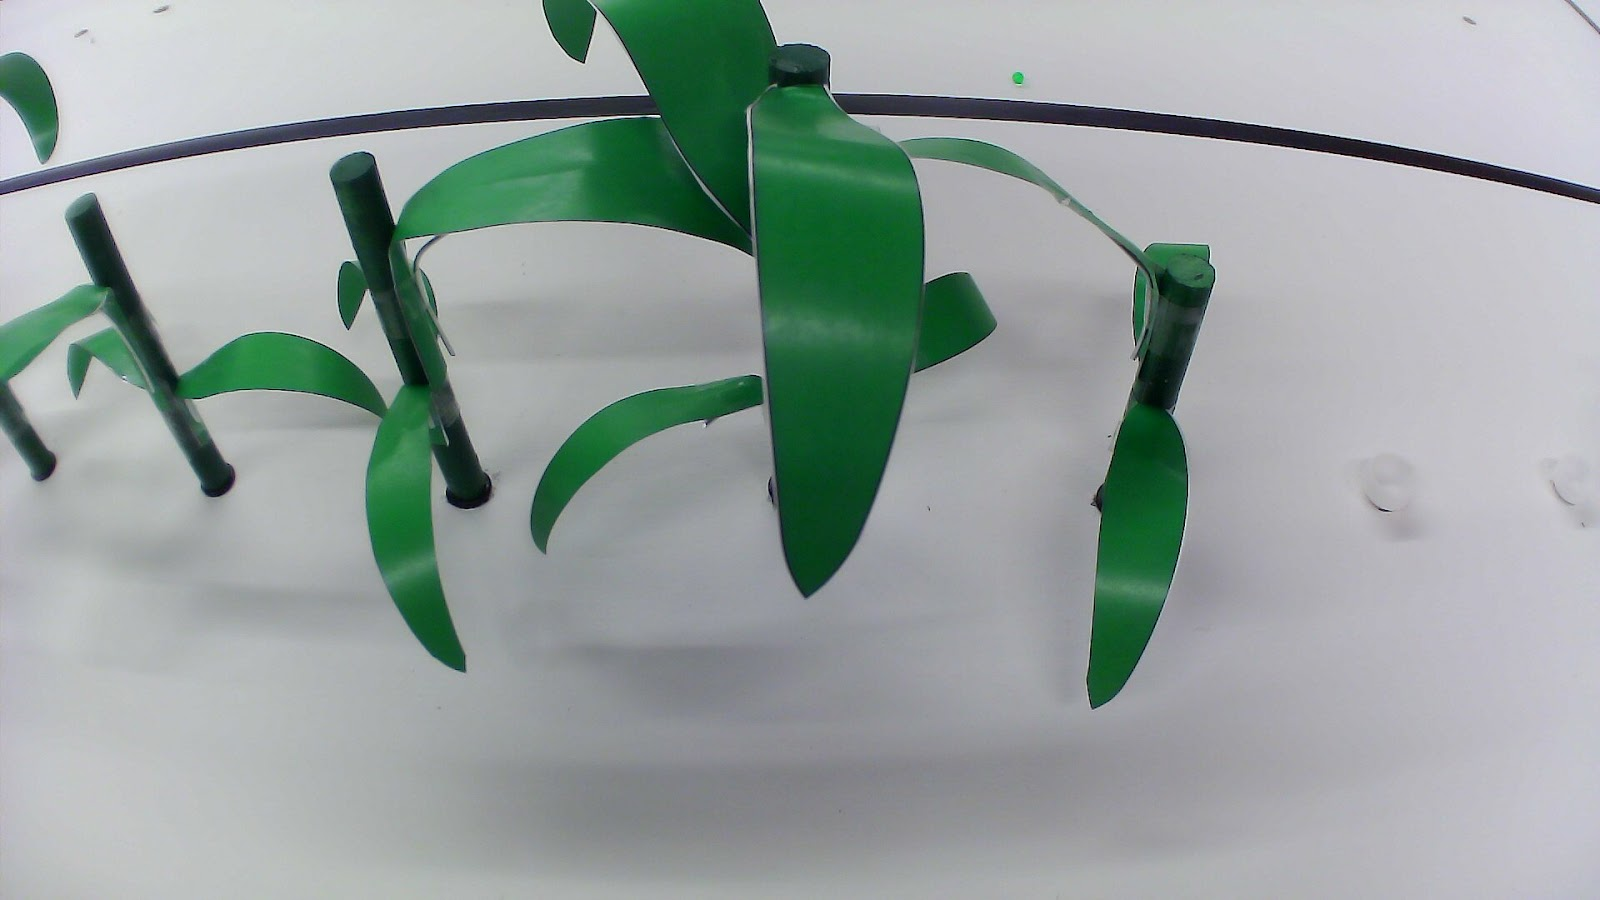
\includegraphics[scale=.2]{uncropped.jpg}
	\end{center}

\subsubsection{Cropped Image} \label{app:crop}
	\begin{center}
	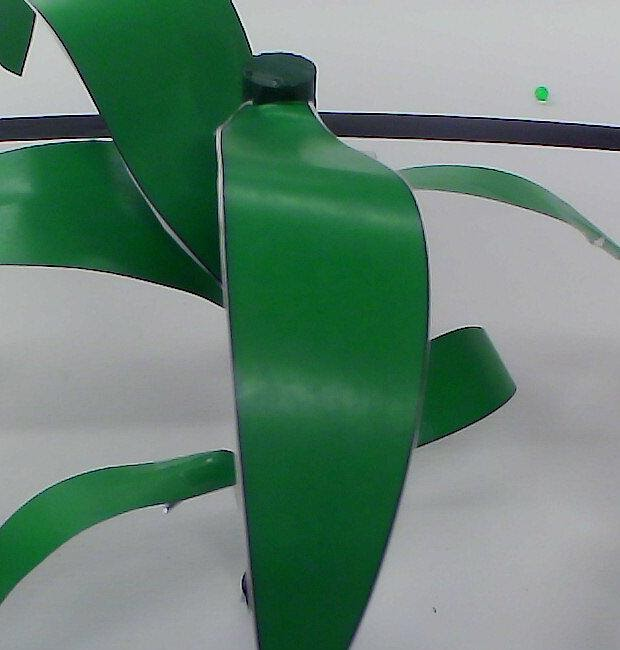
\includegraphics[scale=.2]{cropped.jpg}
	\end{center}
	
\subsubsection{Video of Original Trigger System} \label{app:ogtrig}
	\begin{center}
	\url{https://youtu.be/Y0aVu4daRNE}
	\end{center}

\subsubsection{Dynamixel Trigger System} \label{app:dyntrig}
	\begin{center}
	\url{https://youtu.be/hV4fYE3qgEY}
	\end{center}

\subsubsection{Initial Image Classification} \label{app:ogimg}
	\begin{center}
	TODO
	\end{center}

\subsubsection{Screenshot of Utility} \label{app:util}
	\begin{center}
	TODO
	\end{center}

\subsubsection{Model Training} \label{app:model}
	\begin{center}
	TODO
	\end{center}


\subsection{Software Systems Integration} \label{app:system}
\subsubsection{Software Systems Diagram} \label{app:sysdiag}
	\begin{center}
	TODO
	\end{center}
	

\end{document}